\documentclass[../rapport.tex]{subfiles}
\graphicspath{{\subfix{ressources/photo_diagrammes/}}}

\begin{document}

		\begin{figure}[h]
				\centering 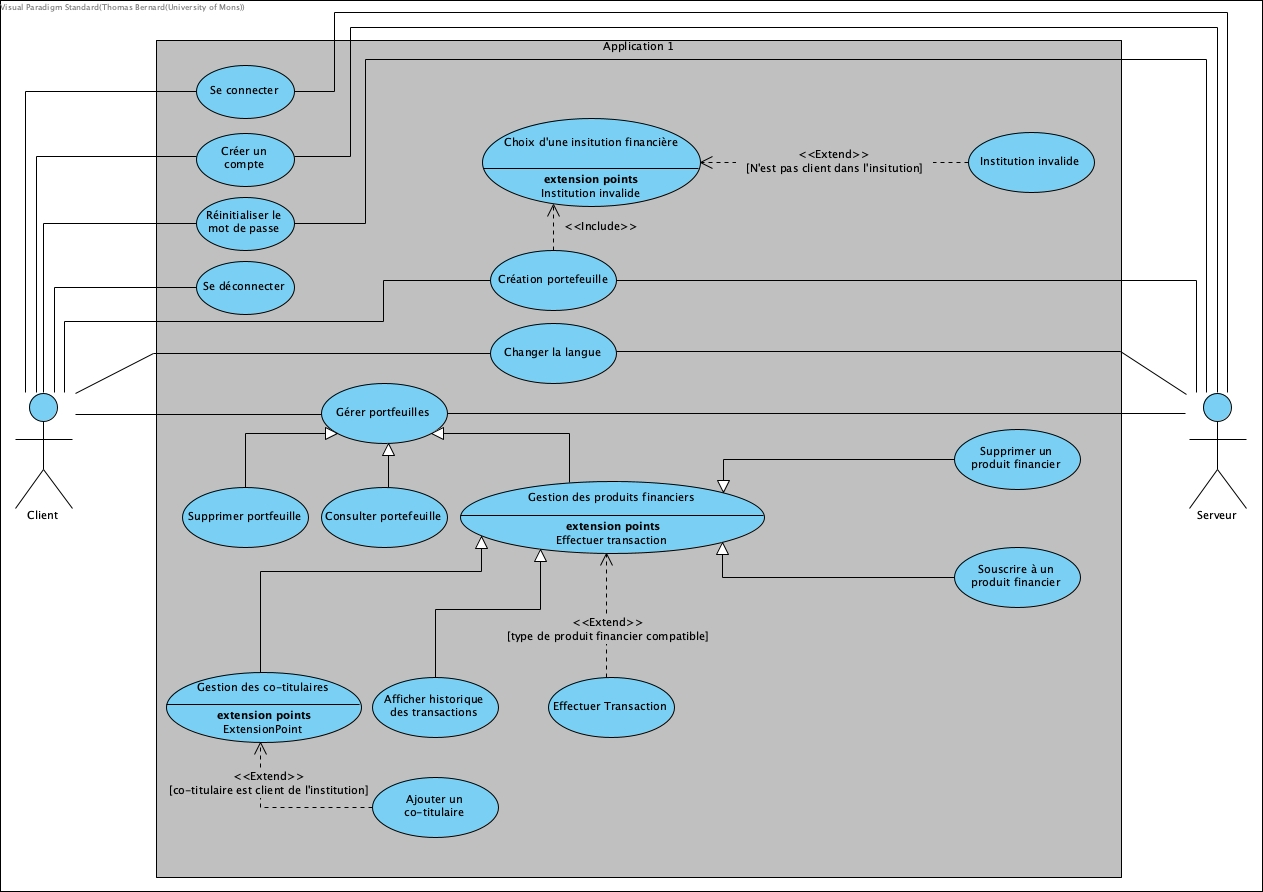
\includegraphics[scale=0.3]{ressources/photos_diagrammes/app1/use_case_app1.jpg}
				\caption{Diagramme des cas d'utilisation de l'Application 1.}
		\end{figure}

		Pour le diagramme de cas d'utilisation nous n'avons pas rencontrés beaucoup de difficultés. Il nous a suffit de lire les consignes du projet et d'en ressortir 
		les points importants qui devaient être les fonctionnalités principales de notre projet. Ce diagramme nous a servi de squelette dans la création de la suite 
		de nos diagrammes. Il n'y a pas remarques importantes à faire à ce sujet car le diagramme ne fait que recenser les actions basiques de l'application 1.
\end{document}
